\documentclass[10pt, aspectratio=169]{beamer}

\include{./../../preamble.tex}
\include{./../../preamble-slides.tex}

\include{./../../tikzlib/preamble.tex}

%\setbeameroption{show notes on second screen=right}

\usepackage{xifthen}

\newcommand{\edaload}[7]{
\fill[lightgray] (#1,#2+0.05) rectangle (#1+#3,#2+0.05+#4/100*0.5);
\draw[thick] (#1,#2+0.05) rectangle (#1+#3,#2+0.55);
\node[inner sep=0pt] (designer) at (#1+#3/2,#2+0.3) {\faUser};

\fill[lightgray] (#1,#2-0.55) rectangle (#1+#3,#2-0.55+#5/100*0.5);
\draw[thick] (#1,#2-0.55) rectangle (#1+#3,#2-0.05);
\node[inner sep=0pt] (machine) at (#1+#3/2,#2-0.3) {\faLaptop};

\ifthenelse{\isempty{#6}}%
  {}%
  {\node[anchor=south] at (#1+#3/2,#2+0.6) {#6};}%


\ifthenelse{\isempty{#7}}%
  {}%
  {
    \draw[thin] (#1,#2-0.65) -- (#1,#2-1);
    \draw[thin] (#1+#3,#2-0.65) -- (#1+#3,#2-1);

    \draw[{Latex[round,scale=0.8]}-{Latex[round,scale=0.8]}] (#1,#2-0.8) -- (#1+#3,#2-0.8)
        node [midway,anchor=north,inner sep=2pt] {#7};
  }
}

\begin{document}

\begin{frame}[fragile]

Kenneth Kundert about the challenges to replace an existing SPICE 
simulator \cite[p. 24]{kundert-lifeafterspice-11}.

\vspace{0.5cm}

\begin{quote}
Designers take great pride in the knowledge that they accumulate at a
great personal cost over the span of their career. 
As such, they are loath to give up their simulator, regardless of how badly it 
has treated them.
\textbf{This is a form of Stockholm syndrome.}
\end{quote}
\end{frame}

\begin{frame}[fragile]
Barrie Gilbert about experience with design automation \cite[p. 39]{gilbert-dfm-02}.

\vspace{0.5cm}

\begin{quote}
\textbf{The writer speaks from painful experience.
In 1960, using an Elliott 803 vacuum-tube computer, he wrote a program for 
The Automatic Design of Circuits.
It really did what it claimed, for a small set of circuits.}
It selected the best devices for a given application out a library of 36 
germanium transistors, and given simple boundary objectives, such as
gain, input noise, bandwidth and the like, it calculated all component values, 
later selecting the nearest available standard values and recalculating the 
bias point and the subsequent effect on the terminal performance.
It then carried out a specified number (the default was 1,000) of 
Monte-Carlo analyses and predicted board (not chip) yield for typical production
variances and their correlation factors.
\textbf{This labour of love was used once or twice, in a
serious capacity, and some examples published in the professional literature.
Then, it fell into oblivion.}
\end{quote}

\end{frame}


\begin{frame}[fragile]
\cite{knuth-taocp1-97}

\vspace{0.5cm}

\begin{quote}
The modern meaning for algorithm is quite similar to
that of recipe, process, method, technique, procedure, routine, rigmarole, 
except that the word “algorithm” connotes something just a little different.
Besides merely being a finite set of rules that gives a sequence of operations 
for solving a specific type of problem, an algorithm has five important 
features.
\end{quote}

\end{frame}

\begin{frame}[fragile]
\cite{knuth-taocp1-97}
\begin{enumerate}
  \item Finiteness (terminate after a finite number of steps)
  \item Definiteness. Each step of an algorithm must be precisely defined; 
    the actions to be carried out must be rigorously and unambiguously 
    specified for each case.
  \item Input. An algorithm has zero or more inputs.
  \item Output. An algorithm has one or more outputs.  
  \item Effectiveness. An algorithm is also generally expected to be effective, 
    in the sense that its operations must all be sufficiently basic that they 
    can in principle be done exactly and in a finite length of time by someone 
    using pencil and paper.
\end{enumerate}
\end{frame}

\begin{frame}[fragile]
\cite{knuth-taocp1-97}

\vspace{0.5cm}

\begin{quote}
A procedure that has all of the characteristics of an algorithm except that it
possibly lacks finiteness may be called a computational method.[...]
Another example of a nonterminating computational method is a reactive process, 
which continually interacts with its environment.[...]
An expression of a computational method in a computer language is called 
a program.
\end{quote}

\end{frame}


\begin{frame}
\frametitle{Quality Aspect}
\begin{columns}
\column{.5\textwidth}

We want
\begin{itemize}
  \item higher speed
  \item lesser power
  \item higher reliability
  \item higher resolution
  \item smaller area
  \item higher accuracy
  \item ...
\end{itemize}

\column{.5\textwidth}

We achieve that by:
\begin{itemize}
  \item technology
  \item architecture
  \item topology
  \item sizing
  \item layout
\end{itemize}
\end{columns}
\end{frame}

\begin{frame}
\frametitle{Productivity Aspect}


\begin{columns}
\column{.5\textwidth}

We want
\begin{itemize}
  \item reduce execution cost (runtime, hardware, licenses)
  \item more accurate results
  \item fewer errors $\rightarrow$ fewer iterations
  \item less manual work
  \item ...
\end{itemize}

\column{.5\textwidth}

We achieve that by:
\begin{itemize}
  \item methods
  \item tools
\end{itemize}
\end{columns}
\end{frame}

\begin{frame}
\frametitle{Taxonomy of EDA-Tools (by example)}

\begin{center}
\begin{tikzpicture}
\input{./../../tikzlib/figs/eda-tools-taxonomy-tree-b.tex}
\end{tikzpicture}
\end{center}
\note[item]{Other manual tool: waveform viewer}
\note[item]{more detailed taxonomy for simulator: analog(SPICE), digital, mixed-signal}
\note[item]{Other analysis tool: PEX, EMIR, constraint verification}
\note[item]{Other synthesis tool: RTL Compiler, floorplanner, LLM}
\note[item]{All automatic tools: setup cost and runtime}
\begin{itemize}
  \item analysis and synthesis tools may are called from a manual tool
  \item a synthesis tool may call an analysis tool several times
\end{itemize}
\end{frame}

\begin{frame}
\frametitle{Human, Time and Financial Resources}
\framesubtitle{Tool Development}

\begin{itemize}
  \item new stuff
  \begin{itemize}
    \item algorithm
    \item hardware interface, e.g. GPU
    \item user interface
    \item assistants
  \end{itemize}

  \item integration
  \begin{itemize}
    \item tools
    \item file formats
  \end{itemize}
\end{itemize}
\end{frame}

\begin{frame}[fragile]
\frametitle{Integration}

\begin{columns}
\column{.25\textwidth}
\begin{center}
designer in the middle

\vspace*{4mm}

\begin{tikzpicture}[scale=.9]
\input{./../../tikzlib/figs/eda-tool-integration-a.tex}
\end{tikzpicture}
\end{center}
\column{.25\textwidth}
\begin{center}
existing frontend

\vspace*{4mm}

\begin{tikzpicture}[scale=.9]
\input{./../../tikzlib/figs/eda-tool-integration-b.tex}
\end{tikzpicture}
\note[item]{Example for \textit{existing frontend}: simulator}
\end{center}
\column{.25\textwidth}
\begin{center}
new frontend

\vspace*{4mm}

\begin{tikzpicture}[scale=.9]
\input{./../../tikzlib/figs/eda-tool-integration-c.tex}
\end{tikzpicture}
\end{center}
\column{.25\textwidth}
\begin{center}
two frontends

\vspace*{4mm}

\begin{tikzpicture}[scale=.9]
\input{./../../tikzlib/figs/eda-tool-integration-d.tex}
\end{tikzpicture}
\note[item]{Example for \textit{two frontends}: DRC, LVS}
\end{center}
\end{columns}
\end{frame}


\begin{frame}
\frametitle{Integration With Non FOSS Tools}

Connecting the new tool with an existing Non FOSS tool

\vspace{5mm}

\begin{itemize}
  \item additional cost, e.g.
    \begin{itemize}
      \item adapter license (Cadence Oasis\footnote{\url{https://semiwiki.com/eda/cadence/2214-cadence-sues-berkeley-design-automation/}})
      \item OpenAccess membership fee (min. \$7,353 per year\footnote{\url{https://si2.org/join-si2/}})
    \end{itemize}  
  \item degree of integration limited, e.g.
    \begin{itemize}
      \item slow (only batch mode)
      \item proprietary programming languages
      \item not all features of a tool are available by API (only GUI)
    \end{itemize}
  \item re-engineering, e.g.
    \begin{itemize}
      \item violation of NDA
      \item may change with each new version
    \end{itemize}
\end{itemize}
\end{frame}

\begin{frame}
\frametitle{Human, Time and Financial Resources}
\framesubtitle{Tool Application}

\begin{itemize}
  \item training
  \item setup
  \item execution
  \begin{itemize}
    \item runtime
    \item hardware
    \item energy
    \item licenses
  \end{itemize}
\end{itemize}

\end{frame}

\begin{frame}
\frametitle{Setup}
\begin{itemize}
  \item for each new PDK (initial and regular updates)
    (related to integration cost)
  \item for each new circuit class (opamp, bandgap,...)
  \item for each new circuit topology (specific netlist or schematic)
  \item for each set of performance parameters (which and how they are extracted)
  \item for each set of performance specification
\end{itemize}

\vspace{5mm}

handle setup cost: specialization, externalization and sharing
\end{frame}

\begin{frame}
\frametitle{Other problems with (new) design automation methods/tools}

\begin{itemize}
  \item productivity when using new method and/or tool first 
    will degrade (valley of pain)

  \item non-design related knowledge needed (algorithms)

  \item designers don't read manuals

  \item designers may focus on what a tool can't do instead what it 
    can do (gotcha problems)

  \item impossible to adapt each new tool (too much variety)

  \item fear of a better option (FOBO)

  \item It is difficult to get a man to understand something, 
    when his salary depends on his not understanding it.
\end{itemize}
\end{frame}

\begin{comment}
\begin{frame}
\frametitle{SPICE Monkeying}

\begin{center}
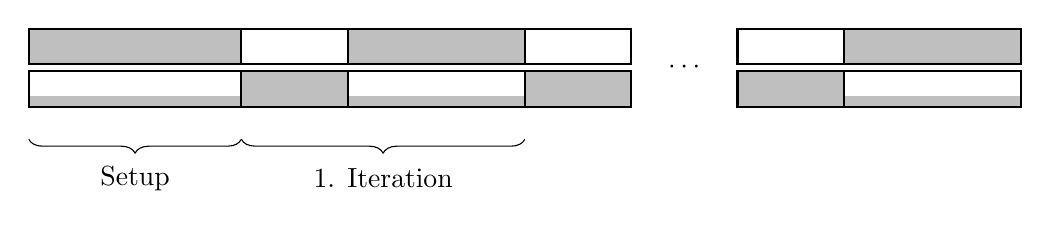
\begin{tikzpicture}[scale=.9]
\edaload{1}{0}{3}{100}{30}{}{}
\edaload{4}{0}{1.5}{0}{100}{}{}
\edaload{5.5}{0}{2.5}{100}{30}{}{}
\edaload{8}{0}{1.5}{0}{100}{}{}

\node[] at (10.25,0) {$\cdots$};

\edaload{11}{0}{1.5}{0}{100}{}{}
\edaload{12.5}{0}{2.5}{100}{30}{}{}

\draw [decorate,decoration={brace,amplitude=5pt,mirror,raise=6ex}]
  (1,0) -- (4,0) node[midway,yshift=-4em]{Setup};
\draw [decorate,decoration={brace,amplitude=5pt,mirror,raise=6ex}]
  (4,0) -- (8,0) node[midway,yshift=-4em]{1. Iteration};


\end{tikzpicture}
\end{center}
\end{frame}
\end{comment}

\begin{frame}
\frametitle{SPICE Monkeying (1)}
\begin{center}
\begin{tikzpicture}[node distance=1.3cm]
\input{./../../tikzlib/figs/spice-monkeying-flowchart-a.tex}
\end{tikzpicture}
\end{center}
\end{frame}

\begin{frame}
\frametitle{SPICE Monkeying (2)}
\begin{columns}[t]
\column{.5\textwidth}

\begin{center}
\textbf{Advantages}
\begin{itemize}
  \item accurate
  \item shared setup cost
\end{itemize}
\end{center}
\column{.5\textwidth}
\begin{center}
\textbf{Disadvantages}
\begin{itemize}
  \item often non-systematic
  \item hard to reproduce
  \item time inefficient
\end{itemize}
\end{center}
\end{columns}
\end{frame}

\begin{frame}
\frametitle{SPICE Monkeying (3)}
\begin{itemize}
  \item[13:42] The phase margin is too low.
  \item[13:44] I will increase the current mirror ratio to fix that.
  \item[13:45] Run simulation.
  \item[13:46] Simulation takes too long, I will check my mails in-between.
  \item[13:50] Finally, simulation is finished.
  \item[13:51] What did I just change?
\end{itemize}
\vspace{5mm}
$\Rightarrow$Delay due to waiting for simulation to finish.
\end{frame}


\begin{frame}[allowframebreaks]
\frametitle{References}
\printbibliography
\end{frame}
\end{document}